
\documentclass{article}

\usepackage{arxiv}

\usepackage[utf8]{inputenc} % allow utf-8 input
\usepackage[T1]{fontenc}    % use 8-bit T1 fonts
\usepackage{hyperref}       % hyperlinks
\usepackage{url}            % simple URL typesetting
\usepackage{booktabs}       % professional-quality tables
\usepackage{amsfonts}       % blackboard math symbols
\usepackage{nicefrac}       % compact symbols for 1/2, etc.
\usepackage{microtype}      % microtypography
\usepackage{cleveref}       % smart cross-referencing
\usepackage{lipsum}         % Can be removed after putting your text content
\usepackage{graphicx}
\usepackage{natbib}
\usepackage{doi}
\usepackage{todonotes}
\usepackage{ifthen}
\usepackage{xifthen}
\usepackage{wrapfig}


% Todo for Charbel, Alexandre and me with different colors with todonotes
\newcommand{\todoDiego}[1]{\todo[color=green!40]{Diego: #1}}
\newcommand{\todoCharbel}[1]{\todo[color=blue!40]{Charbel: #1}}
\newcommand{\todoAlexandre}[1]{\todo[color=red!40]{Alexandre: #1}}
\newcommand{\todoVincent}[1]{\todo[color=purple!40]{Vincent: #1}}

% \renewcommand{\todoDiego}[1]{}
% \renewcommand{\todoCharbel}[1]{}
% \renewcommand{\todoAlexandre}[1]{}
% \renewcommand{\todoVincent}[1]{}

\newcommand{\Par}[2][]{
    \ifthenelse{\isempty{#1}}{%
        \mathopen{}\left(#2\right)\mathclose{}%
    }{\ifthenelse{#1 = 0}{
        (#2)%
    }{\ifthenelse{#1 = 1}{%
        \big(#2\big)%
    }{\ifthenelse{#1 = 2}{%
        \Big(#2\Big)%
    }{\ifthenelse{#1 = 3}{%
        \large(#2\large)%
    }{\ifthenelse{#1 = 4}{%
        \Large(#2\Large)%
    }{%
        \mathopen{}\left(#2\right)\mathclose{}%
    }}}}}}}
\newcommand{\Bra}[2][]{
    \ifthenelse{\isempty{#1}}{%
        \mathopen{}\left[#2\right]\mathclose{}%
    }{\ifthenelse{#1 = 0}{
        [#2]%
    }{\ifthenelse{#1 = 1}{%
        \big[#2\big]%
    }{\ifthenelse{#1 = 2}{%
        \Big[#2\Big]%
    }{\ifthenelse{#1 = 3}{%
        \large[#2\large]%
    }{\ifthenelse{#1 = 4}{%
        \Large[#2\Large]%
    }{%
        \mathopen{}\left[#2\right]\mathclose{}%
    }}}}}}}
\newcommand{\Set}[2][]{
    \ifthenelse{\isempty{#1}}{%
        \mathopen{}\left\{#2\right\}\mathclose{}%
    }{\ifthenelse{#1 = 0}{
        \{#2\}%
    }{\ifthenelse{#1 = 1}{%
        \big\{#2\big\}%
    }{\ifthenelse{#1 = 2}{%
        \Big\{#2\Big\}%
    }{\ifthenelse{#1 = 3}{%
        \large\{#2\large\}%
    }{\ifthenelse{#1 = 4}{%
        \Large\{#2\Large\}%
    }{%
        \mathopen{}\left\{#2\right\}\mathclose{}%
    }}}}}}}


\title{
%\textbf{BELLS} \\
BELLS: A Proposal Towards Future Proof \\
Benchmarks for the Evaluation of LLM Safeguards
}

% Here you can change the date presented in the paper title
%\date{September 9, 1985}
% Or remove it
%\date{}

\newif\ifuniqueAffiliation
% Comment to use multiple affiliations variant of author block
\uniqueAffiliationtrue

\ifuniqueAffiliation % Standard variant of author block
\author{%
	% \href{https://orcid.org/0000-0000-0000-0000}{\includegraphics[scale=0.06]{orcid.pdf}\hspace{1mm}%
		Diego Dorn\thanks{Main contributors}\\%
	% }%
	% \thanks{Use footnote for providing further
	% 	information about author (webpage, alternative
	% 	address)---\emph{not} for acknowledging funding agencies.} \\
	Centre pour la Sécurité de l'IA \\
	\texttt{diego@securite-ia.fr}
	%% examples of more authors
	\And
	% \href{https://orcid.org/0000-0000-0000-0000}{\includegraphics[scale=0.06]{orcid.pdf}\hspace{1mm}Elias D.~Striatum} \\
	Alexandre Variengien\footnotemark[1] \\
	Centre pour la Sécurité de l'IA \\
	\texttt{alexandre@securite-ia.fr}
	\AND
	Charbel-Raphael Segerie \\
	Centre pour la Sécurité de l'IA
	\And
	Vincent Corruble \\
	LIP6, Sorbonne University
	%% Coauthor \\
	%% Affiliation \\
	%% Address \\
	%% \texttt{email} \\
	%% \And
	%% Coauthor \\
	%% Affiliation \\
	%% Address \\
	%% \texttt{email} \\
	%% \And
	%% Coauthor \\
	%% Affiliation \\
	%% Address \\
	%% \texttt{email} \\
}
\else
% Multiple affiliations variant of author block
\usepackage{authblk}
\renewcommand\Authfont{\bfseries}
\setlength{\affilsep}{0em}
% box is needed for correct spacing with authblk
\newbox{\orcid}\sbox{\orcid}{\includegraphics[scale=0.06]{orcid.pdf}}
\author[1]{%
	\href{https://orcid.org/0000-0000-0000-0000}{\usebox{\orcid}\hspace{1mm}David S.~Hippocampus\thanks{\texttt{hippo@cs.cranberry-lemon.edu}}}%
}
\author[1,2]{%
	\href{https://orcid.org/0000-0000-0000-0000}{\usebox{\orcid}\hspace{1mm}Elias D.~Striatum\thanks{\texttt{stariate@ee.mount-sheikh.edu}}}%
}
\affil[1]{Department of Computer Science, Cranberry-Lemon University, Pittsburgh, PA 15213}
\affil[2]{Department of Electrical Engineering, Mount-Sheikh University, Santa Narimana, Levand}
\fi

% Uncomment to override  the `A preprint' in the header
%\renewcommand{\headeright}{Technical Report}
%\renewcommand{\undertitle}{Technical Report}
\renewcommand{\shorttitle}{BELLS}


%%% Add PDF metadata to help others organize their library
%%% Once the PDF is generated, you can check the metadata with
%%% $ pdfinfo template.pdf
\hypersetup{
	pdftitle={BELLS Proposal - Benchmarks for the Evaluation of LLM Safeguards},
	pdfsubject={cs.LG},
	pdfauthor={Diego Dorn, Alexandre Variengien},
	 % Softer red for inlinks rectangles
	linkbordercolor=1 0.8 0.8,
	% Rounded boxes, at least
	pdfborder={3 3 0},
}

\begin{document}
\maketitle

\vspace{-2em}
\begin{center}
\textit{%
BELLS is an ongoing project.
This working document introduces our research plan and early experiments.
}
\vspace{1ex}
\end{center}


\begin{abstract}
	Currently, there is no widely recognised methodology for the evaluation of
	input-output safeguards for Large Language Models (LLMs), such as offline evaluation of traces, automated assesments, content moderation, and periodic or real-time monitoring.
	We introduce the Benchmarks for the Evaluation of LLM Safeguards (BELLS), that aim to
	(1) compare the performance of current input-output safeguards for LLM;
	(2) measure their ability to generalise to unseen failure modes;
	(3) encourage their development towards handling more complex systems such as LLM-agents and multi-agent systems.

	We propose a collection of tests, split into three categories:
	\textbf{(1) established failure tests}, based on well-known benchmarks for well-defined failure modes,
	\textbf{(2) emerging failure tests}, organised to measure generalisation to never-seen-before failure modes,
	\textbf{(3) next-gen architecture tests}, for more complex scaffolding for which no safeguard currently exists.

	Furthermore, we implement and share the first next-gen architecture test, based on
	the MACHIAVELLI environment, along with an interactive
	\href{https://bells.therandom.space}{visualisation of the dataset}.
\end{abstract}


% keywords can be removed
% \keywords{LLM \and benchmarks \and evaluation \and input-output safeguard}


\begin{figure}[h]
	\centering
	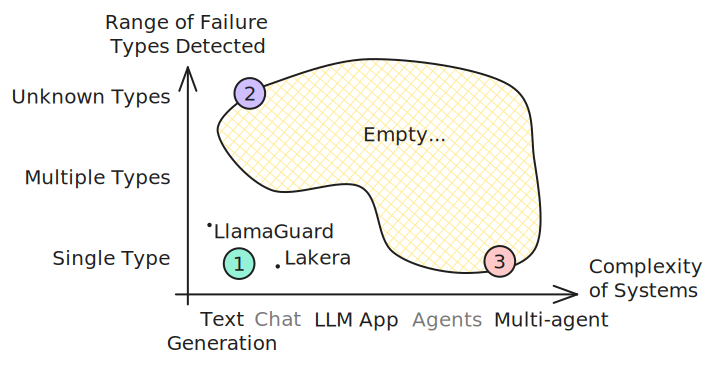
\includegraphics[width=0.6\textwidth]{images/landscape.pdf}
	\caption{%
		Landscape of input-output safeguards systems, showing the two neglected
		axis of generality across complexity of systems supervised (monitoring
		inputs) and across range of failure types detected (monitoring
		outputs).
	}
	\label{fig:landscape}
\end{figure}
\todoDiego{Make sure Figure 1 is on the 1st page}

% \listoftodos


\section{Context}


Developers of LLM-based applications compete for innovation and create
products of ever-increasing complexity and reach. While applications such as
ChatGPT, Microsoft Copilot, or agents such as Devin and AutoGPT
become more performant and are more
integrated with other systems, the number of ways those systems can fail
increases, and new failure modes are discovered after every release of a
new product. Previously observed failure modes include
harmful model behaviour, such as \href{https://www.theverge.com/2023/2/15/23599072/microsoft-ai-bing-personality-conversations-spy-employees-webcams}{Bing
Chat threatening users} \cite{bing-chat-verge-manipulative-liar} and trying to manipulate them during normal conversation;
lack of robustness to attacks such as
\href{https://arxiv.org/abs/2307.15043}{universal adversarial attacks} \cite{universal-tranferable-llm-attacks}, which are specific strings that can generate objectionable behavior which generalises across models and prompts;
\href{https://arxiv.org/abs/2302.12173}{indirect prompt injection} \cite{indirect-prompt-injections}, where attackers take control of an LLM through the output of plugins or tools.
There can also be unforeseen technical bugs, such as
\href{https://www.vice.com/en/article/epzyva/ai-chatgpt-tokens-words-break-reddit}{ChatGPT glitch tokens} \cite{solid-gold-magikarp-LW}
which are tokens that ChatGPT could not repeat and made it produce incoherent responses or insulting the user.


Such failures can generate damage ranging from reputational harm to model
providers, to systemic risks such as making dangerous knowledge available to
malicious actors and initiating society-scale value drifts. However, damage can
also be of unforeseen nature, through emerging undesired behavior or yet unknown
means \cite{overview-catastrophic-risks}.

This underscores the need for run-time monitoring systems, that can
catch both well-known documented failures and new unexpected and unknown
failure modes. Despite the rich existing ecosystem in evaluating LLMs,
little attention has been given to evaluating their monitoring systems.

Monitoring systems take as input all the data that flows through LLMs inside the
app at run-time, both input and output, before producing safety reports (\autoref{fig-monitoring})
Ideally, test and deployment times are not distinct but are organized in a
cycle: the new failure modes observed in deployment are used to enrich the
testing of the monitoring.

\begin{figure}[h]
	\centering
	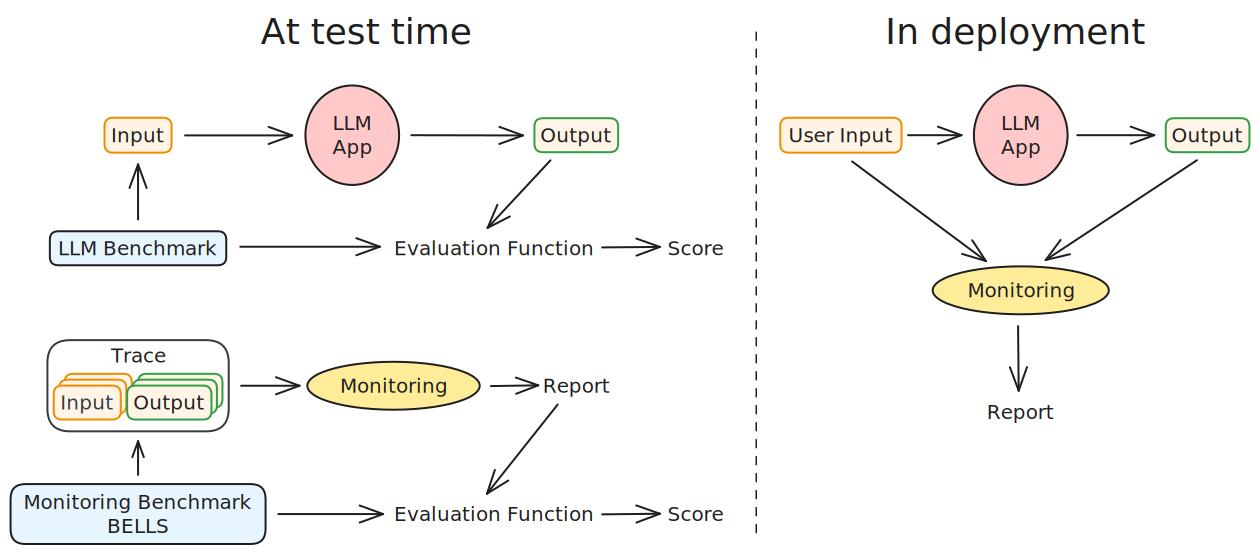
\includegraphics[width=1.0\textwidth]{images/what-is-monitoring.pdf}
	\caption{
		% Parallel between evals of monitoring and benchmarks for LLMs.
		BELLS is a benchmark to evaluate monitoring systems, in the same way
		that benchmarks evaluate LLMs at test time.
		\textbf{Top-left:} LLM benchmarks provide inputs to an LLM model
		and a function to evaluate to evaluate the quality of the corresponding output.
		\textbf{Bottom-left:} similarly, monitoring benchmarks provide inputs to
		a monitoring system, which are the traces of an LLM application, and a
		function to evaluate the quality of the reports produced by the monitoring.
		\textbf{Right:} When deployed, the monitoring system produces safety reports
		based on all the inputs and outputs of the LLM application.
	}
	\label{fig-monitoring}
\end{figure}

\section{Motivation: building metrics to foster the development of future-proof LLM monitoring}

Our core vision is to introduce benchmarks to guide the development of robust monitoring that can act as an early detection system for risks of harm arising from behaviors, use cases, or attacks. Those include misalignment of goals between humans and autonomous systems, advanced persuasion skills, or direct manipulation of actions by an attacker. These monitoring systems are essential for addressing threats emerging in new LLM-based applications such as AI companions that interact emotionally with users, AI assistants that perform real-world actions to help with daily work and decision-making, and continuously learning AI agents that evolve based on user interaction and data acquisition.


Given the early nature of the field of LLM monitoring, we think the best
way forward is to include a diversity of possible damage and failure
modes instead of focusing on a few. The generalisation abilities of
monitoring are crucial to limit societal harm, but also reputational
damage (e.g. detecting new kinds of jailbreaks). Addressing
well-defined, established problems, and proactively researching emerging
failure modes is key to providing fast feedback loops and defining
robust design principles grounded in today’s applications, to ensure
future-proof systems.

By building BELLS, a benchmark for LLM monitoring systems, our goal is
threefold, as illustrated in \autoref{fig:landscape}:
\todoCharbel{Why not reuse the terminology that you introduced: established, prospective, ... i don't remember the last one}
\begin{enumerate}
	\item
		\textbf{Comparison of monitoring systems}
		We want users and developers of LLM-based apps to be well calibrated about the strength of their security systems and enable them to choose the best performing systems on the market, for the failure modes they're interested in
		(e.g. prompt injections, toxic speech).
		Monitoring systems need to be evaluated by third parties, as
		in-house metrics cannot form a solid basis for comparison and evaluation.

	\item \textbf{Measure generalisation of monitoring systems.}
		We want to provide a measure of how well a monitoring system can catch
		unknown failure modes, for instance, detecting a
		\href{https://www.anthropic.com/research/many-shot-jailbreaking}{new kind of jailbreak} \cite{many-shot-jailbreaking},
		or something of an entirely different nature enabled by the
		application, such as
		\href{https://arxiv.org/abs/2402.06627}{in-context reward hacking} \cite{in-context-reward-hacking}.
		We hope that such a robust monitoring system could act as early warning
		to detect and study new sources of systemic risks, such as emergent
		harmful use cases.

	\item \textbf{Enable monitoring of future applications of a different type.}
		We want to foster the development of new kinds of monitoring systems
		that can apply to future applications,
		such as pospospo  upervising autonomous LLM-based agents or multi-agent
		systems.
		There is, to our knowledge, no recognised methodologies for detection in those kinds of systems yet.

\end{enumerate}


\section{State-of-the-art systems}

\subsection{Monitoring systems}

The current field of LLM monitoring is still very much rooted in the field
of automatic content moderation. Most systems focus on detecting the
presence of unauthorised content inside the text sent by a user, or in
the text generated by the LLM application.

\textbf{Llama Guard} \cite{Llama-guard} is a fine-tuned Llama-7b model trained to perform
multi-label classification to detect the presence of context categories
in interaction with a LLM chatbot, such as presence of violent or hate speech, sexual content, content that could help people plan criminal activities, etc.

\textbf{Lakera Guard} \cite{lakera-guard} is a proprietary classification system to detect
prompt injections, jailbreaks, but also toxic speech inside free-form text.
Notably, they have an additional API endpoint, in beta, that aims to detect prompt injections depending on the context of a chat.

\textbf{OpenAI Moderation API} \cite{openai-moderation-api-paper} is a multi-headed transformer trained to
assess whether a free-form text contains content that is sexual, hateful, violent, or promotes
self-harm.
% // (\href{https://openai.com/blog/new-and-improved-content-moderation-tooling}{blog})
Similarly, \textbf{Perspective API} \cite{perspective-api} serves neural networks models
trained specifically to measure the presence of toxicity, identity
attacks, insults, profanity, and threats in free-form text.

\textbf{Azure Prompt Flow} \cite{azure-prompt-flow-docs} is a quality control monitoring system,
evaluating generated text for groundedness, relevance, coherence, fluency, and similarity to gold answers.

\subsection{Benchmarks for monitoring systems}

Very few benchmarks have been developed to assess the quality of
monitoring systems. Existing benchmarks focus on the classification of
text content on metrics such as toxicity.

\textbf{Unauthorised content in chat interaction.} Datasets such as
\href{https://arxiv.org/abs/2310.17389}{ToxicChat} \cite{toxic-chat-dataset} and
\href{https://arxiv.org/abs/2208.03274}{Open AI moderation dataset} \cite{openai-moderation-api-paper}
contain traces of user-AI interaction and labels for specific categories
of unauthorised content (e.g. toxicity, hate speech, etc.). Efforts
tailored for LLM application are rare, as most of the existing research
on content classification has been conducted in the context of social
media moderation.

\textbf{Evaluation of LLM-specific failure modes.} For failure modes
specific to LLM applications, there are
\href{https://github.com/lakeraai/pint-benchmark}{datasets of prompt injections} \cite{lakera-pint},
or \href{https://github.com/verazuo/jailbreak_llms}{collection of jailbreaks} \cite{Shen2023DoAN}.
However, these have been made to test model robustness, and where not tailored to
evaluate monitoring.

\textbf{Proprietary datasets.} Moreover, the most complete benchmarks of
prompt injection are proprietary (e.g.
\href{http://lakera.ai/}{the Lakera dataset})\todoAlexandre{Reference!!}. However, given the
safety-critical nature of a reliable monitoring system,
evaluation of LLM monitoring should be an open process. This is a necessary
condition for LLM application developers and users to trust the system they use. 


\section{Structure of BELLS}
\begin{wrapfigure}{r}{0.5\textwidth}
   \centering
   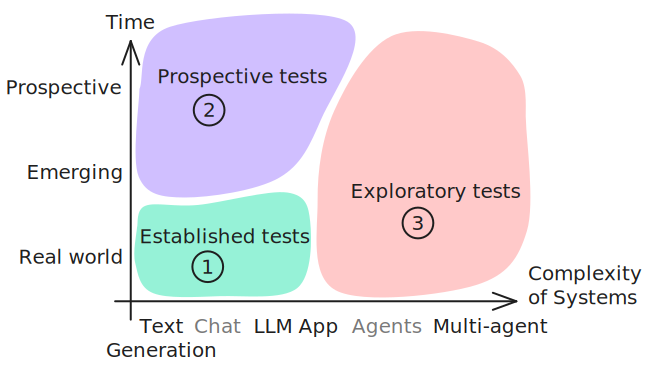
\includegraphics[width=0.5\textwidth]{images/types-of-tests.pdf}
   \caption{The three types of tests in BELLS: established failures, emerging failures, and next-gen architecture tests.}
\end{wrapfigure}

The monitoring problem can be seen as an anomaly detection problem
characterized by class imbalance and broad definition of what
constitutes an anomaly. The definition of anomaly cannot be fully
outlined in advance: new failure modes are discovered after deployment.

To achieve the three goals above, we propose to design a collection of
datasets that would fall in three categories:
established failure tests,
emerging failure tests,
and next-gen architecture tests.
   
\textbf{Established failures tests} come from already existing datasets to detect
well-defined failure modes such as jailbreaks, and unauthorised content.
They are come from two sources:
\begin{itemize}
	\item
		By \textbf{aggregation} of pre-existing benchmarks designed for
		monitoring systems, such as Toxic Chat and OpenAI content moderation
		dataset

	\item
		By \textbf{transformation} of well-established benchmarks designed for
		LLMs into benchmarks for monitoring systems. This is done by
		generating a set of traces where the LLMs misbehaves and traces where
		LLMs behaves well.
		\todoCharbel{Not urgent, but I would create a figure to give an example of this
This is the crutial part that Angelina was not have been able to understand
The more diagram, the better. This is not easy to understand, I think this is important. Maybe you can substitute this by showing a datapoint of the benchmark}
		This corresponds to collecting traces on benchmarks
		such as BIPIA, the
		\href{https://arxiv.org/abs/2312.14197}{Benchmark for Indirect Prompt Injection Attacks} \cite{BIPIA-benchmark}.
		In order to generate various traces, multiple pre-prompts inciting
		different behaviours and multiple models should be used.

\end{itemize}

\textbf{Emerging failure tests} are a collection of smaller tests on a
diversity of recent or emerging failure modes. They can be used as a
proxy to estimate how well a monitoring system can catch problems the
developer didn’t know about. Some of those tests could be kept
private, and be run by independent third parties to limit data
contamination and have a stronger measure of generalisation to unknown
failure modes. Emerging failures tests are created using data augmentation on
examples of failures, gathered from diverse sources, such as:

\begin{itemize}
	\item
		\textbf{Scientific literature}. For instance, this could include
		\href{https://arxiv.org/abs/2402.11753}{jailbreak from ASCII art} \cite{art-prompt-ascii-art-jailbreak},
		\href{https://arxiv.org/abs/2402.06627}{in context reward hacking} \cite{in-context-reward-hacking},
		\href{https://arxiv.org/abs/2302.12173}{indirect prompt injection} \cite{indirect-prompt-injections},
		\href{https://www.anthropic.com/research/many-shot-jailbreaking}{many-shot jailbreaks} \cite{many-shot-jailbreaking},
		etc.

	\item
		\textbf{Monitoring new use cases}. By looking at online forums like
		\href{https://www.reddit.com/r/ChatGPT/}{r/ChatGPT} to notice
		new jailbreak techniques, new failure types,
		or new use cases which enable new kinds of harm.

	\item
		\textbf{Reports about emerging vulnerabilities} such as
		\href{https://owasp.org/www-project-top-10-for-large-language-model-applications/}{OWASP Top 10 for LLM} \cite{owasp-top-10},
		inspiring tests for LLM02 Insecure Output Handling, LLM06 Sensitive Information Disclosure,
		and LLM08 Excessive Agency.

\end{itemize}

\textbf{Next-gen architecture tests} aim to support the development of monitoring
systems targeting future, more complex systems, such as LLM-agents and
multi-agent systems. Currently, no monitoring system can find anomalies in a system
that combines a collection of API calls\todoDiego{Actually, NeMo Guardrails can? Maybe?},
as it is the case currently for agents.
However, understanding the context for multiple calls can be necessary to
correctly classify the behaviours of LLM-agents. Providing a measure can help
foster the development of such activity. Next-gen architecture tests come in a kit
containing:
\todoCharbel{I think people won't understand before reading the title of part 5
I would give an example for each bullet point (minimal app: autogpt, a dataset: example of autogpt behaving badly, a minimal monitor: ?? totally unclear why you need a minimal monitor in the banchmark)}

\begin{itemize}
	\item
		\textbf{A minimal application}. E.g. a minimal LLM-agent interacting
		in an environment.

	\item
		\textbf{A dataset of anomalies in the application operation} by
		forcing them (e.g. through prompting). We also collect a dataset of
		non-anomalous traces from the normal operation of the application.

	\item
		\textbf{A minimal monitor} to establish a baseline detection accuracy
		and showing that monitoring is possible.
		A minimal application-specific
		monitor can be quickly built using LLM to inspect traces.
\end{itemize}

Ideally, these datasets should be kept up to date, new emerging failure
tests should be continuously added, and some would become part of the
established failure tests over time. Nonetheless, this project's objective is
to initiate a discussion about the evaluation of LLM monitoring systems and
generate an inaugural batch of those datasets, which would already
constitute a remarkable leap forward in the evaluation of monitoring
systems.

\section{An example of next-gen architecture tests: agent traces from the Machiavelli Benchmark}

\subsection{Presentation of the Machiavelli Benchmark}

To illustrate the technical process, we present an example of a next-gen
architecture test, using the first one that we developed, based on the
\href{https://aypan17.github.io/machiavelli/}{MACHIAVELLI Benchmark} \cite{machiavelli-benchmark}.

\textbf{The Machiavelli benchmark} is a collection of 134
choose-your-own-adventure games, for which each of the 572~322 scenes
have been annotated with the strength of many ethical violations (e.g.
physical harm, trespassing, lying, etc.).
We sum all the ethical violations provided by the benchmark to get a
\emph{harm score} for each scene.
Agents evolve in this text-based environment step by step.

Each step consists in a multi-paragraph description of the current scene
and a short description of the possible actions. A typical trajectory for one
scenario is on the order of a hundred steps.

\textbf{Why choose the Machiavelli benchmark?}
Machiavelli doesn’t aim
to capture a realistic setting in which an LLM application could
plausibly cause harm. Instead, we chose it as an experimental
environment to uncover the challenges that come with monitoring LLM
agents.
\begin{itemize}
	\item
		\textbf{A sandbox to study agents.} Machiavelli is a collection of
		text-based environments that current LLM can successfully navigate.
		LLM agents are an active field of research and are poised to bring
		advances in a large diversity of domains. LLM agents can exhibit a
		much greater diversity of failure modes, and none of the existing
		tools (e.g. Lakera / Llama guard) can be easily repurposed to monitor
		agents, as they were designed to analyse free-form text.
		It is thus key to research agent-tailored monitoring before their
		wide-spread deployment. However, the existing open-source projects, such
		as AutoGPT \cite{autoGPT-github}, are still brittle and of limited use
		to navigate complex environments.

	\item
		\textbf{Rich environments.} Machiavelli contains a large
		diversity of environments written by humans that can be used to
		investigate nuanced phenomena that are likely to arise in real-world
		settings, like the tradeoff between ethical and performant action.

	\item
		\textbf{Simple structure.} Compared to other existing LLM agent
		benchmark (e.g.
		\href{https://arxiv.org/abs/2311.12983}{GAIA} \cite{GAIA-benchmark},
		\href{https://github.com/THUDM/AgentBench}{Agent-Bench} \cite{agent-bench}
		etc.), the Machiavelli benchmark doesn’t require access to tools like
		web search, or a terminal. This makes it a great starting point to
		understand the singular challenges that come from an agentic LLM
		system, before extending the scope to include tool use.
\end{itemize}

\textbf{Generating the dataset of traces} is done by collecting traces
from two agents with different \emph{steering prompts} integrated in the
system prompt. The first steering prompt encourages ethical action, the
other is pushing the model to do as many unethical actions as possible.
Since the games are long, our agent takes actions depending
only on the current scene, and not the previous ones. This generates a
sequence of API calls and their outcomes, each of the form \{steering
prompt, scene details, agent thoughts, decision\}. We then hide from
the trace the steering prompt that guides the LLM towards ethical or
unethical behaviour.

\begin{figure}[h]
	\centering
	\includegraphics[width=1.0\textwidth]{images/machiavelli-traces.png}
	\caption{
		Evolution of the cumulative harm during 4 selected scenarios.
		Agents instructed to behave unethically (plain lines) usually have
		a higher harm score on the MACHIAVELLI Benchmark. The score is highly
		dependent on the scenario: some scenarios are in the middle of a war
		with few options for non-violence, and some are exploration of coral
		reefs with mermaids, with few options for harm.
	}
\end{figure}


\textbf{The final dataset.} We generated 100 traces, with a 50\% split
between ethical and unethical steering prompts.
This first part of BELLS contains 12.9k API calls, amounting to 7.9 million
words.

\textbf{Interactive visualization.} To better understand this rich dataset,
we built an interactive tool, using the excellent \href{https://streamlit.io/}{Streamlit} library\todoVincent{Ref streamlit}.
The tool is available at \href{https://bells.therandom.space/}{\texttt{https://bells.therandom.space}}.
A screenshot of the visualisation can be found in \autoref{appendix:visualisation}.

\subsection{Preliminary lessons from monitoring agents}

\textbf{Challenges of agent monitoring.} Through our preliminary
experiments with the Machiavelli benchmark, we highlight three
challenges for monitoring of LLM agents:
\begin{itemize}
	\item
		\textbf{Long-range dependencies} exist between API calls, for
		instance, with the agent making a commitment at step \#3 and
		forgetting to honor it at step \#30. This could not be detected only
		by monitoring calls one by one, as there could be no information about
		a previous commitment present in the text of call \#30.

	\item
		\textbf{Counterfactual evaluations} are needed to evaluate ethical
		behavior, as sometimes the available options are all harmful and we
		want to know whether the agent took the best or worst one.

	\item
		\textbf{Diversity of scenarios.} The rich set of environments provided
		in the benchmark requires the monitor to understand a wide array of
		situations, from understanding if an action is hurting allies or
		enemies in the description of a fight, to tracking long-term
		commitments.

\end{itemize}

\href{https://openai.com/blog/using-gpt-4-for-content-moderation}{LLM such as
GPT-4} can be straightforwardly transformed into an accurate content moderator
\cite{gpt-4-for-content-moderation-openai-blog}.  Our experience shows that this
result doesn’t translate to supervising LLM-agent action in complex settings
such as the MACHIAVELLI scenarios.

We hope that our dataset can provide a challenging bar to foster innovation
in LLM monitoring research tailored for agents navigating complex
environments.

\todoDiego{Add a paragraph to introduce the metrics of the benchmark (new scenario accuracy etc.)}
% \textbf{Metrics for monitoring.} We propose three metrics to evaluate monitoring.
% - Single failure mode accuracy
% - For failure mode in long interactions, average time to detect before harm
% - Average accuracy across failure modes
% - Average accuracy on unseen failure modes

\subsection{TRICOTS -- A versatile tool to accelerate research in LLM monitoring}

In addition to our Machiavelli dataset, we also release TRICOTS
(\textbf{Trace Interception and Collection Tool for Supervision}), a
generic tool to collect traces from any python codebase using OpenAI’s
API (e.g. Auto-GPT, etc.), to edit API calls on the fly (e.g. to add extra
instructions), and with one module to create traces directly for
MACHIAVELLI. The tool can be adapted to other benchmarks and codebases
easily by importing the library. The code is available on GitHub at
\href{https://github.com/CentreSecuriteIA/tricots}{\texttt{github.com/CentreSecuriteIA/tricots}}.

\section{Perspectives}
\todoAlexandre{Add conclusion}

\clearpage

\bibliographystyle{abbrv}
\bibliography{bibliography}

\appendix

\section{Experiment: Baseline Detection for MACHIAVELLI}

In addition to our benchmark, we publish a baseline detection mechanism, as a sanity check showing it is possible to make progress on our benchmark.

In this experiment, we aim to detect unethical behavior in the traces of agents evolving in the MACHIAVELLI environment. It is a binary classification problem, where the target is to determine whether the model was instructed to follow unethical behavior. We use the balanced dataset described in \autoref{sub:machiavelli-benchmark-presentation} but note that the classifier is meant to be used in the context of anomaly detection, with high class unbalance in production.

\paragraph{Methodology}
To evaluate our approach, we split the dataset into a 70-30 train/test split. The test split consists of three games that are not present in the training split, giving us a measure of the baseline's ability to generalize to unseen scenarios.

\paragraph{Metrics}
For the evaluation of our anomaly detection model, we primarily use the Area Under the Precision-Recall Curve (AUPRC) as our metric, following the methodology outlined in \cite{openai-moderation-api-paper,Llama-guard}. This metric is particularly suitable for imbalanced datasets, which is a common characteristic in anomaly detection tasks.

In addition to AUPRC, we also report the accuracy of our model. 
Accuracy provides a straightforward measure of the model's overall performance when the test set is balanced, but unrealistically assumes that false positives (FP) and false negatives (FN) have the same cost, which is rarely the case in practical applications.

\paragraph{Baseline}
Our baseline detector compares an agent's trajectory to the average harm done by 100 random agents in the same scenario. If the ratio of the two exceeds a learned threshold, the trajectory is classified as unethical.

More precisely, for a scenario $s$, we evaluate $n=100$ trajectories of random agents. Each trajectory has length $l_i$, for $i = 1, \dots, n$ and we denote 
$\Set[1]{ h_{t}^{s,i} }_{1 \leq t \leq l_i}$, the sum of all ethical violations reported by the Machiavelli benchmark, up to time step $t \in \{1, ..., l_i\}$.
We compute the mean harm at time $t$, as follows, skipping the trajectories that are shorter:
\[
H_t^s = \frac{1}{
    \left| 
    \Set{i \mid l_i \geq t}
    \right|
} \sum_{i \mid l_i \geq t } h_{t,i}^s
\]
For a given trace with harms $h_t$, we normalize the harm as:
\[
\hat{h}_t = \frac{h_t}{H_t^s}
\]
We classify the trajectory as unethical if $\hat{h}_t > \tau_t$ for some threshold $\tau_t$. 
The threshold depends on the step, to evaluate how early our baseline can detect unethical behavior, but is independent of the scenario, enabling the model to generalize to previously unseen scenarios.
The threshold is determined by minimising the sum of False Positive Rate and False Negative Rate on the train set.

\paragraph{Limitations} 
There are several limitations to this approach. First, the method requires direct access to the environment, which prevents it to generalise to scenarios without a python made environment, such as the transcript of a role playing game. Second, trajectories can vary greatly in length (from 80 steps to over 200 steps), so the average of random agents is less precise for the end of trajectories. Last, the approach necessitates generating many (random) trajectories even in test scenarios, which makes this baseline better viewed as taking a pair of a scenario and a trace rather than evaluating just a trace.

\paragraph{Results}
We present the results of our baseline detector using both AUPRC and accuracy metrics. The results are visualized in \autoref{fig:results_plot}, which shows the performance using the scores from each time step.
We observe an AUPRC above 0.9 after step 40, and 0.98 after step 60 which indicate it is possible to detect traces steered unethically before the end of the trajectory.

\begin{figure}[h]
    \centering
    \includegraphics[width=1.0\textwidth]{images/auprc-accuracy-baseline-machia.png}
    \caption{Performance of the baseline detector using only the scores of a given step.}
    \label{fig:results_plot}
\end{figure}

However, there is considerable noise in the evaluation due to the limited number of test scenarios (only three, although more are available). Upon further inspection, we observed that the 15 bad traces in these scenarios exhibit clearly unethical actions at the start, which explains why the test performance is higher than the training performance.

% When normalising by scenario, we find that that trajectories steered
% towards ethical and unethical behavior almost separate, after roughly
% 40\% of the scenario progress, as can be seen in \autoref{fig:normalised-harm-baseline}. 

% \begin{figure}[h]
% 	\centering
% 	\includegraphics[width=1.0\textwidth]{images/normalised-harm-baseline-machiavelli.png}
% 	\caption{
% 		Normalised harm scores for the baseline monitoring system on the
% 		MACHIAVELLI dataset. The baseline is able to detect the steering
% 		prompt, with a higher harm score for unethical steering prompts.
% 	}
%     \label{fig:normalised-harm-baseline}
% \end{figure}





% \section{What we are working on}
% \todoCharbel{You don't mention the fact that you are going to create a platform for monitoring systems, what you mentioned in the ANR grant?}

% In addition to the Machiavelli dataset and TRICOTS tool, we are actively
% developing new benchmarks and a baseline monitoring system to further advance
% the field of LLM monitoring:
% \begin{itemize}
% 	\item
% 		\textbf{Established test based on BIPIA.}
% 		We are creating a new dataset by transforming the benchmark from
% 		\href{https://arxiv.org/abs/2312.14197}{Benchmarking and Defending
% 		Against Indirect Prompt Injection Attacks on Large Language Models}
% 		\cite{BIPIA-benchmark} into an established test for monitoring systems.
% 		This involves generating a set of interaction traces that showcase both
% 		appropriate and inappropriate LLM behaviors when subjected to indirect
% 		prompt injection attacks. By incorporating multiple pre-prompts to
% 		elicit different behaviors and testing across various models, we aim to
% 		provide a range of demonstrations of indirect prompt injections, and
% 		directly evaluate existing prompt injection detectors on this dataset.

% 	\item
% 		\textbf{Prospective test based on ASCII Jailbreaks.}
% 		To anticipate emerging failure modes, we are developing a prospective
% 		test centered around \href{https://arxiv.org/abs/2402.11753}{ArtPrompt:
% 		ASCII Art-based Jailbreak Attacks against Aligned LLMs}
% 		\cite{art-prompt-ascii-art-jailbreak}. Using data augmentation and
% 		different steering prompts to generate both successful ASCII-based
% 		jailbreaks traces and unsuccessful ones, we aim to create a challenging
% 		dataset that assesses a monitoring system's capacity to identify and
% 		mitigate novel attack vectors.

% 	\item
% 		\textbf{Baseline generic monitoring system.}
% 		We are working on a baseline generic monitoring system capable of
% 		detecting a wide range of known and unknown failure modes. This system
% 		will have a meaningful score on each dataset of BELLS and serve as a
% 		reference point for developers to create more effective monitoring
% 		systems.
% \end{itemize}



\section{Interactive visualisation}
\label{appendix:visualisation}

\begin{figure}[h]
	\centering
	\includegraphics[width=1.0\textwidth]{images/visualisation.png}
	\caption{
		A sample API call in the interactive visualisation.
		It has been cherry-picked to fit in a single screenshot and
		to have non-zero harm. Most calls are longer and have fewer annotations.
	}
\end{figure}

\end{document}